\documentclass[a4paper,11pt]{amsart}

% =========================================================================
%  Informe de laboratorio — Práctica 1: Momento de inercia. Teorema de Steiner
%  Estilo: el del informe del efecto Doppler (artículo científico
%  minimalista, Palatino, versalitas, enunciados numerados por sección,
%  paleta de azules y grises), con los encabezados de sección, el índice y
%  la paginación inspirados en el guion de Cosmosofía.
% =========================================================================

% --- IDIOMA Y CODIFICACIÓN ------------------------------------------------
\usepackage[utf8]{inputenc}
\usepackage[T1]{fontenc}
\usepackage[spanish,es-tabla,es-nodecimaldot]{babel}

% --- TIPOGRAFÍA (Palatino) --------------------------------------------------
\usepackage{mathpazo}
\linespread{1.05}
\usepackage[final]{microtype}

% --- MATEMÁTICAS Y UNIDADES ------------------------------------------------
\usepackage{amsmath, amssymb, mathtools}
\usepackage{bm}
\usepackage{siunitx}
\sisetup{
  output-decimal-marker = {,},
  group-minimum-digits  = 4,
  group-digits          = integer,
  group-separator       = {\,},
  per-mode              = symbol,
  separate-uncertainty  = true,
  range-phrase          = {\text{ a }},
  detect-all            = false
}

% --- PÁGINA, COLORES Y GRÁFICOS --------------------------------------------
\usepackage[a4paper,margin=2.6cm]{geometry}
\usepackage{graphicx}
\usepackage{xcolor}
\definecolor{azulprof}{HTML}{1B365D}    % azul marino
\definecolor{azulacero}{HTML}{3B6EA8}   % azul acero
\definecolor{azulclaro}{HTML}{B7CBE3}   % azul hielo
\definecolor{grispizarra}{HTML}{5B6770} % gris pizarra
\definecolor{grisclaro}{HTML}{E4E8EC}   % gris perla
\definecolor{azulfondo}{HTML}{F3F7FB}   % fondo tenue de referencias y resultados
\definecolor{acento}{HTML}{B8800A}      % acento sobrio (ámbar oscuro) para comparaciones
\usepackage{tikz}
\usetikzlibrary{babel, arrows.meta, calc, positioning, decorations.pathmorphing,
                decorations.markings, patterns}
\usepackage{pgfplots}
\pgfplotsset{compat=1.17}
\usepackage{booktabs}
\usepackage{multirow}
\usepackage[most]{tcolorbox}
\usepackage{array}
\usepackage{enumitem}
\setlist[itemize]{leftmargin=1.6em, itemsep=2pt, topsep=4pt}
\setlist[enumerate]{leftmargin=1.8em, itemsep=2pt, topsep=4pt}

% --- ENLACES Y REFERENCIAS CRUZADAS ----------------------------------------
\usepackage[colorlinks=true, linkcolor=azulacero, citecolor=azulacero,
            urlcolor=azulacero, plainpages=false, pdfusetitle=false,
            pdftitle={Práctica 1: Momento de inercia. Teorema de Steiner},
            pdfauthor={David Gómez García; Daniel Martín Guerrero}]{hyperref}
\usepackage[spanish,nameinlink]{cleveref}

% --- BIBLIOGRAFÍA -----------------------------------------------------------
\usepackage{csquotes}
\usepackage[backend=biber, style=numeric, sorting=none, giveninits=true,
            maxbibnames=6, minbibnames=3, doi=true, url=true,
            isbn=false]{biblatex}
\addbibresource{referencias.bib}
\DeclareFieldFormat[article,techreport,unpublished]{title}{#1\isdot}
\DeclareFieldFormat{url}{\url{#1}}
\renewcommand*{\bibfont}{\small}
\setlength{\bibitemsep}{3pt}

% --- PIEZAS DE DIBUJO DEL PÉNDULO DE TORSIÓN ---------------------------------
%%%%%%%%%%%%%%%%%%%%%%%%%%%%%%%%%%%%%%%%%%%%%%%%%%%%%%%%%%%%%%%%%%%%%%%%
% Piezas de dibujo del péndulo de torsión en perspectiva (TikZ)
%
% Proyección oblicua sencilla: un punto (x,y,z) del espacio se dibuja en
%   (x, \kp*y + z),
% de modo que el plano horizontal se ve «tumbado» (como las órbitas de la
% portada de Cosmosofía) y el eje vertical conserva su longitud.
% Se usan en la portada y en la figura del montaje experimental.
%%%%%%%%%%%%%%%%%%%%%%%%%%%%%%%%%%%%%%%%%%%%%%%%%%%%%%%%%%%%%%%%%%%%%%%%

\def\kp{0.40}   % factor de achatamiento del plano horizontal

% --- Muelle espiral (espiral de Arquímedes en el plano z = #4) -------------
% \muelle{r_min}{r_max}{vueltas}{z}: cada vuelta se dibuja como una cinta
% metálica (trazo oscuro con alma clara), algo más intensa hacia fuera.
\newcommand{\muelle}[4]{%
  \pgfmathsetmacro{\mb}{(#2-#1)/(2*pi*#3)}%
  \pgfmathtruncatemacro{\mn}{ceil(#3)-1}%
  \foreach \k in {0,...,\mn}{%
    \pgfmathsetmacro{\ta}{2*pi*\k}%
    \pgfmathsetmacro{\tb}{min(2*pi*(\k+1),2*pi*#3)}%
    \pgfmathsetmacro{\pc}{45+55*\k/max(\mn,1)}%
    \draw[azulprof!\pc!azulclaro, line width=2.3pt, line cap=round]
      plot[domain=\ta:\tb, samples=90, variable=\t, smooth]
      ({(#1+\mb*\t)*cos(\t r)}, {\kp*(#1+\mb*\t)*sin(\t r)+#4});
    \draw[white, line width=0.8pt, line cap=round, opacity=0.85]
      plot[domain=\ta:\tb, samples=90, variable=\t, smooth]
      ({(#1+\mb*\t)*cos(\t r)}, {\kp*(#1+\mb*\t)*sin(\t r)+#4});
  }}

% --- Elipse horizontal (circunferencia de radio #1 en el plano z = #2) ----
\newcommand{\anillo}[3][]{%
  \draw[#1] (0,#3) ellipse [x radius=#2, y radius=\kp*#2];}

% --- Cilindro ensartado en la varilla -------------------------------------
% \cilindro{s}{theta}{h}{rho}{l}: cilindro de radio rho y semilongitud l,
% con su eje a lo largo de la dirección theta del plano z = h y centro a
% distancia s del eje de giro.  Se dibuja la cara oculta, el cuerpo (entre
% las dos generatrices de contorno) y la cara visible.
\newcommand{\cilindro}[5]{%
  \pgfmathsetmacro{\cs}{cos(#2)}\pgfmathsetmacro{\sn}{sin(#2)}%
  \pgfmathsetmacro{\cx}{#1*\cs}\pgfmathsetmacro{\cy}{\kp*#1*\sn+#3}%
  \pgfmathsetmacro{\dx}{#5*\cs}\pgfmathsetmacro{\dy}{#5*\kp*\sn}%
  % semiejes conjugados de las caras: u = rho(-sin, k cos), v = rho(0, 1)
  \pgfmathsetmacro{\ua}{-#4*\sn}\pgfmathsetmacro{\ub}{#4*\kp*\cs}%
  % parámetro de las generatrices de contorno: tan t0 = cos(theta)/k
  \pgfmathsetmacro{\tz}{atan2(\cs,\kp)}%
  \pgfmathsetmacro{\ex}{\ua*cos(\tz)}\pgfmathsetmacro{\ey}{\ub*cos(\tz)+#4*sin(\tz)}%
  % cara visible: la que mira hacia el observador (normal con y < 0)
  \pgfmathsetmacro{\sv}{ifthenelse(\sn>0,-1,1)}%
  \coordinate (cV) at ({\cx+\sv*\dx},{\cy+\sv*\dy});
  \coordinate (cO) at ({\cx-\sv*\dx},{\cy-\sv*\dy});
  \draw[azulprof, line width=0.5pt, fill=azulclaro!70]
    [cm={\ua,\ub,0,#4,(cO)}] (0,0) circle (1);
  \fill[azulclaro!70]
    ($(cO)+(\ex,\ey)$) -- ($(cV)+(\ex,\ey)$) -- ($(cV)-(\ex,\ey)$) -- ($(cO)-(\ex,\ey)$) -- cycle;
  \draw[azulprof, line width=0.5pt] ($(cO)+(\ex,\ey)$) -- ($(cV)+(\ex,\ey)$);
  \draw[azulprof, line width=0.5pt] ($(cO)-(\ex,\ey)$) -- ($(cV)-(\ex,\ey)$);
  \draw[azulprof, line width=0.6pt, fill=azulfondo]
    [cm={\ua,\ub,0,#4,(cV)}] (0,0) circle (1);
  \fill[azulprof] [cm={\ua,\ub,0,#4,(cV)}] (0,0) circle (0.16);
}

% --- Tramo de varilla en el plano z = h, a lo largo de la dirección theta --
% \varilla{theta}{s1}{s2}{h}
\newcommand{\varilla}[4]{%
  \pgfmathsetmacro{\va}{#2}\pgfmathsetmacro{\vb}{#3}%
  \draw[grispizarra, line width=2.1pt, line cap=round]
    ({\va*cos(#1)},{\kp*\va*sin(#1)+#4}) -- ({\vb*cos(#1)},{\kp*\vb*sin(#1)+#4});
  \draw[grisclaro, line width=0.7pt, line cap=round]
    ({\va*cos(#1)},{\kp*\va*sin(#1)+#4+0.012}) -- ({\vb*cos(#1)},{\kp*\vb*sin(#1)+#4+0.012});}

% --- Péndulo de torsión completo -------------------------------------------
% \pendulotorsion{phi}{h}{R}{L}: muelle en z = 0, varilla de semilongitud L
% girada un ángulo phi en el plano z = h y cilindros a distancia R del eje.
% El orden de trazado resuelve las ocultaciones: tramo exterior trasero,
% cilindro trasero, tramo central, eje y tuerca, cilindro delantero y tramo
% exterior delantero.
\newcommand{\pendulotorsion}[4]{%
  \def\rc{0.52}\def\lc{0.62}%
  % eje de giro bajo el muelle (hacia el soporte) y muelle espiral
  \draw[grispizarra!70, line width=2.4pt] (0,-1.9) -- (0,0);
  \muelle{0.42}{4.3}{4}{0}
  % sujeción del extremo exterior del muelle
  \fill[grispizarra] (4.18,-0.16) rectangle (4.52,0.20);
  \draw[grispizarra!70, line width=1.4pt] (4.35,-0.16) -- (4.35,-1.25);
  % cubo central y eje hasta la varilla
  \draw[azulprof, fill=white, line width=0.5pt] (0,0) ellipse [x radius=0.42, y radius=\kp*0.42];
  \draw[grispizarra, line width=2.6pt] (0,0) -- (0,#2);
  \draw[grisclaro, line width=0.8pt] (-0.02,0.05) -- (-0.02,#2);
  % varilla y cilindros
  \varilla{#1}{#3+\lc}{#4}{#2}
  \cilindro{#3}{#1}{#2}{\rc}{\lc}
  \varilla{#1}{#3-\lc}{-#3+\lc}{#2}
  % tuerca de sujeción sobre el eje
  \fill[grispizarra!90] (-0.17,#2) rectangle (0.17,#2+0.42);
  \fill[grispizarra!90] (0,#2+0.42) ellipse [x radius=0.17, y radius=\kp*0.17];
  \fill[grispizarra!60] (0,#2+0.42) ellipse [x radius=0.10, y radius=\kp*0.10];
  \cilindro{#3}{#1+180}{#2}{\rc}{\lc}
  \varilla{#1+180}{#3+\lc}{#4}{#2}
}


% =========================================================================
%        CABECERAS, PIE DE PÁGINA, SECCIONES E ÍNDICE (aire de Cosmosofía)
% =========================================================================
% Pequeña espiral: viñeta de la paginación y ornamento entre secciones
\newcommand{\espiralita}[1][0.9]{%
  \tikz[baseline=-0.6ex, scale=#1]{%
    \draw[azulacero, line width=0.45pt]
      plot[domain=0:15.7, samples=70, variable=\t, smooth]
      ({0.0105*\t*cos(\t r)},{0.0105*\t*sin(\t r)});
    \fill[azulprof] (0,0) circle (0.55pt);}}
\newcommand{\ornamento}{%
  \par\vspace{10pt}{\centering
  \tikz{\draw[azulclaro, line width=0.4pt] (-1.6,0) -- (-0.32,0);
        \draw[azulclaro, line width=0.4pt] (0.32,0) -- (1.6,0);
        \node at (0,0) {\espiralita[1.6]};}\par}\vspace{6pt}}

\makeatletter
\def\ps@headings{%
  \let\@mkboth\markboth
  \def\@evenhead{\normalfont\footnotesize\color{grispizarra}\scshape
    \textls[60]{Laboratorio de Mecánica y Ondas}\hfil
    \textls[60]{Momento de inercia\,\textperiodcentered\,Teorema de Steiner}}%
  \let\@oddhead\@evenhead
  \def\@evenfoot{\hfil\normalfont\small\color{azulacero}%
    \espiralita\enspace\thepage\enspace\espiralita\hfil}%
  \let\@oddfoot\@evenfoot}
\def\ps@firstpage{\ps@plain\def\@oddhead{}\let\@evenhead\@oddhead
  \def\@oddfoot{\hfil\normalfont\small\color{azulacero}%
    \espiralita\enspace\thepage\enspace\espiralita\hfil}%
  \let\@evenfoot\@oddfoot}
\pagestyle{headings}

% Secciones: número en azul acero, título en versalitas espaciadas; debajo,
% un subtítulo en cursiva y un filete rematado en un pequeño círculo.
\def\section{\@startsection{section}{1}%
  \z@{1.3\linespacing\@plus.8\linespacing}{.25\linespacing}%
  {\normalfont\Large\color{azulprof}\scshape\lsstyle\raggedright}}
\let\@seccntformatorig\@seccntformat
\def\@seccntformat#1{%
  \ifnum\pdfstrcmp{#1}{section}=\z@
    {\color{azulacero}\upshape\csname the#1\endcsname}\hspace{0.55em}%
  \else\@seccntformatorig{#1}\fi}
\newcommand{\filete}{%
  \tikz[baseline]{\draw[azulclaro, line width=0.45pt] (0,0) -- (\linewidth-5pt,0);
    \draw[azulacero, line width=0.5pt, fill=white] (\linewidth-2.6pt,0) circle (2.3pt);}}
\DeclareRobustCommand{\tocsub}[1]{%
  \ \textperiodcentered\ {\itshape\color{grispizarra}#1}}
\newcommand{\subtitulo}[1]{%
  \par\nopagebreak\vspace{-2pt}%
  \noindent{\itshape\color{grispizarra}#1}\par\nopagebreak\vspace{1pt}%
  \noindent\filete\par\nopagebreak\vspace{0.55\baselineskip}}
% \seccion{Título}{Subtítulo}: sección numerada con subtítulo (índice incluido).
% amsart escribe en el índice el título principal, no el opcional, así que el
% subtítulo se añade a esa entrada mediante \@tocextra.
\let\@tocextra\@empty
\def\@tocwriteb#1#2#3{%
  \begingroup
    \def\@tocline##1##2##3##4##5##6{%
      \ifnum##1>\c@tocdepth
      \else \sbox\z@{##5\let\indentlabel\@tochangmeasure##6}\fi}%
    \csname l@#2\endcsname{#1{\csname#2name\endcsname}{\@secnumber}{}}%
  \endgroup
  \addcontentsline{toc}{#2}%
    {\protect#1{\csname#2name\endcsname}{\@secnumber}{#3\@tocextra}}%
  \global\let\@tocextra\@empty}
\newcommand{\seccion}[2]{%
  \gdef\@tocextra{\tocsub{#2}}%
  \section{#1}\subtitulo{#2}}

% Índice: número en azul acero, título en azul marino y subtítulo en cursiva
\def\l@section{\@tocline{1}{7pt}{0pt}{}{}}
\renewcommand{\tocsection}[3]{%
  \indentlabel{\@ifnotempty{#2}{{\color{azulacero}#2}\quad}}{\color{azulprof}#3}}
\def\l@subsection{\@tocline{2}{1pt}{1.55pc}{2.4pc}{\small}}
\renewcommand{\contentsnamefont}{\scshape\color{azulprof}\lsstyle}
\makeatother
\numberwithin{equation}{section}
\setcounter{tocdepth}{2}
\makeatletter
\def\@@and{y}
\renewcommand{\keywordsname}{Palabras clave}
\renewcommand{\abstractname}{\color{azulacero}\lsstyle Resumen}
\makeatother

% =========================================================================
%               NOTACIÓN Y MACROS DE USO FRECUENTE
% =========================================================================
\newcommand{\Icm}{I_{\mathrm{CM}}}            % momento de inercia respecto al CM
\newcommand{\Ib}{I_{\mathrm{b}}}              % varilla (barra)
\newcommand{\Ic}{I_{\mathrm{c}}}              % un cilindro móvil
\newcommand{\Ie}{I_{\mathrm{e}}}              % eje y piezas de sujeción
\newcommand{\mb}{m_{\mathrm{b}}}
\newcommand{\mc}{m_{\mathrm{c}}}
\newcommand{\dif}{\mathrm{d}}
\newcommand{\ddt}[1]{\frac{\dif #1}{\dif t}}
\newcommand{\vect}[1]{\vec{#1}}
\newcommand{\Tcoef}{t_{95,\nu}}               % factor de cobertura al 95 %
\newcommand{\ext}[1]{U(#1)}                   % incertidumbre ampliada
\newcommand{\mean}[1]{\overline{#1}}
% Dato pendiente de incorporar (se resalta con discreción)
\newcommand{\pend}[1]{\textcolor{grispizarra}{\colorbox{grisclaro}{\strut\,#1\,}}}
\newcommand{\pendiente}[1]{\textcolor{grispizarra}{\textit{[#1]}}}
% Hueco reservado para una gráfica o figura que aún no existe
\newcommand{\huecofigura}[2][5.2cm]{%
  \tikz{\draw[grispizarra!45, dashed, line width=0.5pt, rounded corners=2pt, fill=azulfondo]
          (0,0) rectangle (0.92\linewidth,#1);
        \node[text=grispizarra, font=\small\itshape, align=center, text width=0.8\linewidth]
          at (0.46\linewidth,#1/2) {#2};}}

% =========================================================================
%        ENTORNOS FORMALES (enunciados numerados, estilo artículo)
% =========================================================================
\usepackage{amsthm}

% Enunciados en cursiva (resultados generales)
\newtheoremstyle{cienplano}{10pt}{10pt}{\itshape}{}%
  {\bfseries\color{azulprof}}{.}{0.6em}%
  {\thmname{#1}\thmnumber{ #2}\thmnote{\normalfont\upshape\ (#3)}}
% Definiciones, cálculos y estimaciones (cuerpo en redonda)
\newtheoremstyle{ciendef}{10pt}{10pt}{\normalfont}{}%
  {\bfseries\color{azulprof}}{.}{0.6em}%
  {\thmname{#1}\thmnumber{ #2}\thmnote{\normalfont\upshape\ (#3)}}
% Observaciones (encabezado en cursiva)
\newtheoremstyle{cienobs}{8pt}{8pt}{\normalfont}{}%
  {\itshape\color{azulprof}}{.}{0.6em}%
  {\thmname{#1}\thmnumber{ #2}\thmnote{\normalfont\upshape\ (#3)}}

\theoremstyle{cienplano}
\newtheorem{proposicion}{Proposición}[section]
\newtheorem{teorema}[proposicion]{Teorema}
\newtheorem{resultado}[proposicion]{Resultado}
\newtheorem{conclusion}[proposicion]{Conclusión}
\theoremstyle{ciendef}
\newtheorem{definicion}[proposicion]{Definición}
\newtheorem{hipotesis}[proposicion]{Hipótesis}
\newtheorem{calculo}[proposicion]{Cálculo de incertidumbre}
\newtheorem{estimacion}[proposicion]{Estimación lineal}
\theoremstyle{cienobs}
\newtheorem{observacion}[proposicion]{Observación}
\newtheorem*{demostracion}{Demostración}

% --- Referencia formalizada --------------------------------------------------
% Caja fina con fondo tenue y título sobre el borde. Cuerpo en cursiva y, al
% pie, la fuente completa con autor, título y número de cita. Comparte
% contador con los enunciados.
% Uso: \begin{referencia}[título]{clave-bib} ... \end{referencia}
\newcounter{referencia}
\renewcommand{\thereferencia}{\theproposicion}
\newtcolorbox{referenciabox}[2]{%
  enhanced, breakable, sharp corners,
  colback=azulfondo, colframe=azulclaro, boxrule=0.4pt,
  left=10pt, right=10pt, top=7pt, bottom=6pt,
  before skip=14pt, after skip=12pt,
  attach boxed title to top left={yshift*=-\tcboxedtitleheight/2, xshift=8pt},
  boxed title style={colback=white, colframe=white, sharp corners, boxrule=0pt,
                     left=3pt, right=3pt, top=1pt, bottom=1pt},
  fonttitle=\bfseries\color{azulprof}, coltitle=azulprof,
  fontupper=\itshape,
  title={Referencia~\thereferencia\ifx\relax#1\relax\else\ \normalfont(#1)\fi},
  after upper={\par\vspace{5pt}{\color{azulclaro}\hrule height 0.4pt}\vspace{4pt}%
    {\upshape\footnotesize\color{grispizarra}\raggedleft
     \citeauthor{#2}, \citetitle{#2}~\cite{#2}.\par}}}
\newenvironment{referencia}[2][]
  {\par\stepcounter{proposicion}\refstepcounter{referencia}\begin{referenciabox}{#1}{#2}}
  {\end{referenciabox}}
\crefname{referencia}{referencia}{referencias}

% --- Método (caja azulada para los fundamentos del tratamiento de datos) -----
\newcounter{metodo}
\renewcommand{\themetodo}{\theproposicion}
\newtcolorbox{metodobox}[1]{%
  enhanced, breakable, sharp corners,
  colback=azulfondo, colframe=azulclaro, boxrule=0.4pt,
  left=10pt, right=10pt, top=7pt, bottom=5pt,
  before skip=14pt, after skip=12pt,
  attach boxed title to top left={yshift*=-\tcboxedtitleheight/2, xshift=8pt},
  boxed title style={colback=white, colframe=white, sharp corners, boxrule=0pt,
                     left=3pt, right=3pt, top=1pt, bottom=1pt},
  fonttitle=\bfseries\color{azulprof}, coltitle=azulprof,
  title={Método~\themetodo\ifx\relax#1\relax\else\ \normalfont(#1)\fi}}
\newenvironment{metodo}[1][]
  {\par\stepcounter{proposicion}\refstepcounter{metodo}\begin{metodobox}{#1}}
  {\end{metodobox}}
\crefname{metodo}{método}{métodos}
\Crefname{metodo}{Método}{Métodos}
\Crefname{referencia}{Referencia}{Referencias}

% --- Resultado destacado ----------------------------------------------------
% Fondo azulado tenue y filete lateral: magnitudes calculadas con su
% incertidumbre.  Uso: \begin{destacado}[rótulo opcional] ... \end{destacado}
\newtcolorbox{destacado}[1][]{%
  enhanced, sharp corners, frame hidden, colback=azulfondo,
  borderline west={1.6pt}{0pt}{azulacero},
  left=10pt, right=8pt, top=2pt, bottom=4pt,
  before skip=8pt, after skip=10pt,
  before upper={\ifx\relax#1\relax\else{\scshape\small\color{azulacero}#1}\par\vspace{-4pt}\fi}}

\crefname{proposicion}{proposición}{proposiciones}
\Crefname{proposicion}{Proposición}{Proposiciones}
\crefname{teorema}{teorema}{teoremas}
\Crefname{teorema}{Teorema}{Teoremas}
\crefname{definicion}{definición}{definiciones}
\Crefname{definicion}{Definición}{Definiciones}
\crefname{resultado}{resultado}{resultados}
\Crefname{resultado}{Resultado}{Resultados}
\crefname{conclusion}{conclusión}{conclusiones}
\crefname{hipotesis}{hipótesis}{hipótesis}
\crefname{calculo}{cálculo}{cálculos}
\crefname{estimacion}{estimación}{estimaciones}
\crefname{observacion}{observación}{observaciones}
\Crefname{observacion}{Observación}{Observaciones}
\crefname{section}{sección}{secciones}
\Crefname{section}{Sección}{Secciones}
\crefname{subsection}{sección}{secciones}
\Crefname{subsection}{Sección}{Secciones}
\crefname{table}{tabla}{tablas}
\Crefname{table}{Tabla}{Tablas}
\crefname{figure}{figura}{figuras}
\Crefname{figure}{Figura}{Figuras}
\crefname{equation}{ecuación}{ecuaciones}
\Crefname{equation}{Ecuación}{Ecuaciones}
\crefformat{equation}{ecuación~(#2#1#3)}
\Crefformat{equation}{Ecuación~(#2#1#3)}
\crefrangeformat{equation}{ecuaciones~(#3#1#4)--(#5#2#6)}
\crefmultiformat{equation}{ecuaciones~(#2#1#3)}{ y~(#2#1#3)}{, (#2#1#3)}{ y~(#2#1#3)}

% --- Estilo de gráficas de datos ----------------------------------------------
\pgfplotsset{
  datos/.style={
    tick label style={font=\scriptsize}, label style={font=\small},
    axis lines=left, axis line style={grispizarra},
    grid=major, grid style={grisclaro, line width=0.4pt},
    every tick/.style={grispizarra},
    legend style={font=\scriptsize, draw=none, fill=white, fill opacity=0.9,
                  text opacity=1, cells={anchor=west}},
    legend cell align=left,
    /pgf/number format/use comma, /pgf/number format/1000 sep={\,},
    scaled ticks=false,
  },
  puntoA/.style={only marks, mark=*, mark size=2.1pt, azulprof,
    mark options={fill=azulprof, draw=white, line width=0.3pt},
    error bars/.cd, y dir=both, y explicit,
    error bar style={line width=0.6pt, azulprof}, error mark options={rotate=90, mark size=2.2pt, line width=0.6pt, azulprof}},
  ajuste/.style={azulprof, line width=1.1pt},
  teorica/.style={acento, line width=0.9pt, densely dashed},
}

% Referencia a un panel de figura: «figura 2\,(a)», enlazada en bloque
\newcommand{\figpanel}[2]{\hyperref[#1]{figura~\ref*{#1}\,\textup{(#2)}}}

% Pies de figura y tabla
\usepackage[font=small, labelfont={sc,color=azulprof}, labelsep=period,
            margin=0.6cm, justification=justified]{caption}

% =========================================================================
%                     VARIABLES PARA LA PORTADA
% =========================================================================
\newcommand{\Universidad}{Universidad de Salamanca}
\newcommand{\Facultad}{Facultad de Ciencias}
\newcommand{\Titulacion}{Grado en Física}
\newcommand{\Asignatura}{Laboratorio de Mecánica y Ondas}
\newcommand{\NumPractica}{Práctica 1}
\newcommand{\TituloPractica}{Momento de inercia\\Teorema de Steiner}
\newcommand{\SubtituloPractica}{Oscilaciones de torsión de un sólido rígido}
\newcommand{\tipotrabajo}{Informe de laboratorio}
\newcommand{\miNombre}{David Gómez García \\ Daniel Martín Guerrero}
\newcommand{\miTutor}{Mario Amado \\ Ivan de Martino \\ Manuel Pino}
\newcommand{\miUbicacion}{Salamanca}

% =========================================================================
%                     DATOS DEL ARTÍCULO (cabecera)
% =========================================================================
\title{Momento de inercia. Teorema de Steiner}
\author{David Gómez García}
\author{Daniel Martín Guerrero}
\address{Grado en Física, Facultad de Ciencias, Universidad de Salamanca,
         Salamanca, España}
\date{}
\keywords{momento de inercia, teorema de Steiner, péndulo de torsión,
constante de torsión, oscilador armónico, regresión lineal}


% =========================================================================
%                                DOCUMENTO
% =========================================================================
\begin{document}
% --- PORTADA ----------------------------------------------------------------
\pagenumbering{alph}
%%%%%%%%%%%%%%%%%%%%%%%%%%%%%%%%%%%%%%%%%%%%%%%%%%%%%%%%%%%%%%%%%%%%%%%%
% Portada — estilo artículo científico, motivo: péndulo de torsión
% Misma cabecera y pie que el informe del efecto Doppler; el dibujo, en
% perspectiva tumbada, rinde homenaje a las órbitas de Cosmosofía.
% Requiere (definidos en main.tex): colores azulprof, azulacero, azulclaro,
% grispizarra, grisclaro, azulfondo; macros \Universidad, \Facultad,
% \Titulacion, \Asignatura, \NumPractica, \TituloPractica,
% \SubtituloPractica, \tipotrabajo, \miNombre, \miTutor, \miUbicacion;
% y figuras/torsion.tex.
%%%%%%%%%%%%%%%%%%%%%%%%%%%%%%%%%%%%%%%%%%%%%%%%%%%%%%%%%%%%%%%%%%%%%%%%

\begin{titlepage}
\thispagestyle{empty}
\pagecolor{white}

\begin{tikzpicture}[remember picture, overlay]
  \coordinate (O) at (current page.south west);

  % ----------------------------------------------------------------
  % Cabecera: logotipos y filete
  % ----------------------------------------------------------------
  \node[anchor=north west, inner sep=0] at ($(O)+(2.2cm,27.9cm)$)
    {
\includegraphics[height=1.42cm]{figuras/logo-usal.png}};
  \node[anchor=north east, inner sep=0] at ($(O)+(18.8cm,27.9cm)$)
    {
\includegraphics[height=1.42cm]{figuras/logo-ciencias.png}};
  \draw[grispizarra!60, line width=0.4pt]
    ($(O)+(2.2cm,26.0cm)$) -- ($(O)+(18.8cm,26.0cm)$);
  \node[anchor=north west, inner sep=0, text=grispizarra, font=\scshape\small]
    at ($(O)+(2.2cm,25.75cm)$)
    {\textls[80]{\Universidad\ \textbar\ \Facultad}};
  \node[anchor=north east, inner sep=0, text=grispizarra, font=\scshape\small]
    at ($(O)+(18.8cm,25.75cm)$)
    {\textls[80]{\Titulacion}};

  % ----------------------------------------------------------------
  % Motivo gráfico: péndulo de torsión visto en perspectiva.
  % Muelle espiral en el plano inferior; varilla con dos cilindros
  % girada un ángulo phi respecto a su posición de equilibrio
  % (discontinua); escala angular y trayectoria de los cilindros.
  % ----------------------------------------------------------------
  \begin{scope}[shift={($(O)+(10.5cm,17.7cm)$)}, x=1cm, y=1cm]
    \def\phiP{24}\def\hP{2.5}\def\RP{5.0}\def\LP{7.1}
    % órbitas tenues y escala angular en el plano de la varilla
    \anillo[azulclaro!55, line width=0.35pt]{7.75}{\hP}
    \anillo[azulclaro!40, line width=0.3pt]{8.35}{\hP}
    \foreach \a in {0,5,...,355}{
      \pgfmathsetmacro{\lt}{ifthenelse(mod(\a,30)==0,0.32,0.14)}
      \draw[azulclaro!90!azulacero, line width=0.35pt]
        ({7.75*cos(\a)},{\kp*7.75*sin(\a)+\hP}) --
        ({(7.75-\lt)*cos(\a)},{\kp*(7.75-\lt)*sin(\a)+\hP});}
    % trayectoria de los centros de los cilindros
    \anillo[azulacero!70, line width=0.5pt, densely dotted]{\RP}{\hP}
    % posición de equilibrio (phi = 0)
    \draw[grispizarra!55, line width=0.6pt, dashed]
      (-\LP,\hP) -- (\LP,\hP);
    % ángulo girado
    \draw[azulacero, line width=0.7pt, -{Stealth[length=5pt]}]
      plot[domain=2:\phiP-1.5, samples=30, variable=\t]
      ({6.55*cos(\t)},{\kp*6.55*sin(\t)+\hP});
    \node[azulprof, font=\large] at ({7.05*cos(\phiP/2)},{\kp*7.05*sin(\phiP/2)+\hP+0.05}) {$\varphi$};
    % el péndulo
    \pendulotorsion{\phiP}{\hP}{\RP}{\LP}
    % distancia R de los cilindros al eje
    \draw[grispizarra, line width=0.45pt, |<->|]
      (0,\hP+1.25) -- ({-\RP*cos(\phiP)},{-\kp*\RP*sin(\phiP)+\hP+1.25})
      node[midway, above=1pt, text=azulprof, fill=white, inner sep=1.5pt] {$R$};
    \draw[grispizarra!50, line width=0.3pt, densely dotted]
      ({-\RP*cos(\phiP)},{-\kp*\RP*sin(\phiP)+\hP+0.6}) --
      ({-\RP*cos(\phiP)},{-\kp*\RP*sin(\phiP)+\hP+1.25});
    % rótulos discretos, al modo de «tú estás aquí»
    \draw[grispizarra!70, line width=0.35pt] (3.2,-0.55) -- (5.3,-1.75);
    \fill[azulacero] (3.2,-0.55) circle (1.3pt);
    \node[anchor=west, text=grispizarra, font=\itshape\small]
      at (5.35,-1.78) {muelle espiral, $D$};
    \draw[grispizarra!70, line width=0.35pt] (0,-1.2) -- (-2.6,-2.05);
    \fill[azulacero] (0,-1.2) circle (1.3pt);
    \node[anchor=east, text=grispizarra, font=\itshape\small]
      at (-2.65,-2.08) {eje de giro};
  \end{scope}

  % ----------------------------------------------------------------
  % Escala de ejes paralelos: I_r = I_CM + m r^2 crece con r^2
  % (como la línea del tiempo de Cosmosofía)
  % ----------------------------------------------------------------
  \begin{scope}[shift={($(O)+(0,13.45cm)$)}, x=1cm, y=1cm]
    \draw[grispizarra!60, line width=0.4pt] (2.2,0) -- (18.8,0);
    \draw[azulacero!60, line width=0.4pt, densely dashed, domain=0:5.25, samples=40]
      plot ({3.0+2.85*\x},{0.22+0.052*\x*\x});
    \foreach \k in {0,...,5}{
      \pgfmathsetmacro{\xk}{3.0+2.85*\k}
      \pgfmathsetmacro{\yk}{0.22+0.052*\k*\k}
      \pgfmathsetmacro{\pc}{30+14*\k}
      \draw[azulprof!\pc!azulclaro, line width=1.3pt] (\xk,0) -- (\xk,\yk);
      \fill[azulprof!\pc!azulclaro] (\xk,\yk) circle (2.1pt);
      \fill[azulprof] (\xk,0) circle (1.2pt);}
    \node[anchor=north, text=grispizarra, font=\itshape\footnotesize] at (3.0,-0.12) {eje por el CM};
    \foreach \k in {1,...,4}{
      \node[anchor=north, text=grispizarra, font=\footnotesize] at ({3.0+2.85*\k},-0.12) {$r_{\k}$};}
    \node[anchor=north, text=grispizarra, font=\itshape\footnotesize] at (17.25,-0.12) {borde del disco};
    \node[anchor=north, text=grispizarra, font=\scshape\scriptsize] at (10.5,-0.62)
      {\textls[160]{momento de inercia respecto a ejes paralelos}};
  \end{scope}

  % ----------------------------------------------------------------
  % Bloque del título
  % ----------------------------------------------------------------
  \node[anchor=north west, inner sep=0, text width=16.6cm, align=left]
    at ($(O)+(2.2cm,11.35cm)$)
    {{\color{azulacero}\scshape\large\textls[120]{\Asignatura\ \textbar\ \NumPractica}}\\[12pt]
     {\color{azulprof}\fontsize{33}{38}\selectfont\bfseries\spaceskip=0.28em\relax\TituloPractica}\\[10pt]
     {\color{azulprof}\itshape\Large\SubtituloPractica}\\[12pt]
     {\color{azulacero}\rule{2.5cm}{1.4pt}}\\[9pt]
     {\color{grispizarra}\large
      $T=2\pi\sqrt{I/D}$
      \quad\textperiodcentered\quad
      $I_{r}=I_{\mathrm{CM}}+m\,r^{2}$}};

  % ----------------------------------------------------------------
  % Pie: tipo de trabajo, autores, tutores, lugar y fecha
  % ----------------------------------------------------------------
  \draw[grispizarra!60, line width=0.4pt]
    ($(O)+(2.2cm,4.6cm)$) -- ($(O)+(18.8cm,4.6cm)$);

  \node[anchor=north west, inner sep=0, text width=4.6cm, align=left]
    at ($(O)+(2.2cm,4.25cm)$)
    {{\scshape\small\color{azulacero}\textls[80]{Documento}}\\[3pt]
     {\large\bfseries\color{azulprof}\tipotrabajo}};

  \node[anchor=north west, inner sep=0, text width=5.6cm, align=left]
    at ($(O)+(7.2cm,4.25cm)$)
    {{\scshape\small\color{azulacero}\textls[80]{Autores}}\\[3pt]
     {\large\color{black!85}\miNombre}};

  \node[anchor=north west, inner sep=0, text width=5cm, align=left]
    at ($(O)+(13.8cm,4.25cm)$)
    {{\scshape\small\color{azulacero}\textls[80]{Tutores}}\\[3pt]
     {\large\color{black!85}\miTutor}};

  \node[anchor=south east, inner sep=0, text=grispizarra, font=\scshape\small]
    at ($(O)+(18.8cm,1.2cm)$)
    {\textls[100]{\miUbicacion, \number\year}};
  \fill[azulprof] ($(O)+(0,0)$) rectangle ($(O)+(21cm,0.45cm)$);
  \fill[azulacero] ($(O)+(0,0)$) rectangle ($(O)+(7cm,0.45cm)$);
  \fill[azulclaro] ($(O)+(0,0)$) rectangle ($(O)+(3cm,0.45cm)$);
\end{tikzpicture}

\end{titlepage}

\clearpage
\pagenumbering{arabic}
\setcounter{page}{1}

\begin{abstract}
Estudiamos las oscilaciones de torsión de distintos sólidos rígidos montados
sobre un eje vertical acoplado a un muelle espiral. En el régimen de pequeñas
oscilaciones el periodo depende únicamente del momento de inercia del cuerpo
y de la constante de torsión del muelle, de modo que medir tiempos con un
cronómetro nos permite medir inercia rotacional. Primero calibramos el muelle
con una varilla y dos cilindros móviles: la pendiente de la regresión lineal
de $T^{2}$ frente a $R^{2}$ proporciona la constante de torsión $D$. Después
comprobamos el teorema de Steiner con un disco perforado, cuyo $T^{2}$ debe
crecer linealmente con el cuadrado $r^{2}$ de la distancia entre el eje de
giro y el centro de masas, y de ese ajuste estimamos la masa del disco y su
momento de inercia respecto al centro de masas. Por último, medimos los
momentos de inercia de una esfera, un cilindro hueco y un cilindro macizo y
los comparamos con sus expresiones teóricas. Los resultados se expresan con su
incertidumbre típica y ampliada al \SI{95}{\percent}, siguiendo \emph{Notes on
Uncertainty in Measurements}.
\end{abstract}

\maketitle
\tableofcontents

% =========================================================================
\newpage
\seccion{Introducción}{La inercia de la rotación}\label{sec:introduccion}
% =========================================================================
La mecánica de la traslación descansa sobre una idea sencilla: la masa mide
cuánto se resiste un cuerpo a cambiar su estado de movimiento. Cuando el
movimiento es de rotación, ese papel lo asume el \emph{momento de inercia},
una magnitud que no depende solo de cuánta masa tiene el cuerpo, sino también
de cómo está repartida alrededor del eje de giro~\cite{FI-FAB,FI-DMG}. Por
eso el patinador que recoge los brazos gira más deprisa, y por eso un mismo
objeto puede resultar fácil o difícil de hacer girar según el eje que
elijamos.

Esa dependencia con el eje es justamente lo que precisa el teorema de
Steiner, o de los ejes paralelos: basta conocer el momento de inercia
respecto a un eje que pase por el centro de masas para conocerlo respecto a
cualquier otro paralelo a él. Es un resultado que hemos usado muchas veces en
los problemas de Física~I; en esta práctica queremos verlo aparecer en el
laboratorio.

Para ello trabajamos con un péndulo de torsión: un eje vertical unido a un
muelle espiral sobre el que se montan distintos cuerpos. Si lo apartamos un
ángulo pequeño de su posición de equilibrio, el sistema oscila con un periodo
que depende solo del momento de inercia del cuerpo y de la constante de
torsión del muelle. Medir tiempos se convierte así en una manera de medir
inercia rotacional~\cite{GUION-P1}.

\subsection{Objetivos}\label{sec:objetivos}
\begin{itemize}
  \item Determinar la constante de torsión $D$ del muelle espiral.
  \item Comprobar el teorema de Steiner con un disco perforado y estimar, a
        partir de él, la masa del disco y su momento de inercia respecto al
        centro de masas.
  \item Determinar los momentos de inercia de una esfera, un cilindro hueco y
        un cilindro macizo, y compararlos con los que predicen sus
        expresiones teóricas.
\end{itemize}
La constante $D$ la obtenemos de la pendiente de una regresión lineal de
$T^{2}$ frente a $R^{2}$ con la varilla y los cilindros móviles
(\cref{eq:varilla}); el teorema de Steiner lo contrastamos con la
linealidad de $T^{2}$ frente a $r^{2}$ para el disco (\cref{eq:steinerT}),
y los momentos de inercia de los sólidos, despejándolos del periodo con la
\cref{eq:periodo}.

\subsection{Material empleado}\label{sec:material}
Para el desarrollo de la experiencia hemos utilizado el siguiente
instrumental (\cref{fig:fotos}):
\begin{itemize}
  \item Muelle espiral con soporte y eje vertical de giro.
  \item Varilla metálica con dos cilindros móviles.
  \item Disco con perforaciones a distintas distancias de su centro.
  \item Sólidos de distinta geometría: esfera, cilindro hueco y cilindro
        macizo.
  \item Cronómetro.
  \item Regla milimetrada, cinta métrica y calibre (pie de rey).
  % \item Balanza (si se han pesado los cuerpos en lugar de usar las masas
  %       indicadas en el laboratorio).
\end{itemize}

\begin{figure}[ht]
\centering
\begin{minipage}[b]{0.235\textwidth}\centering
  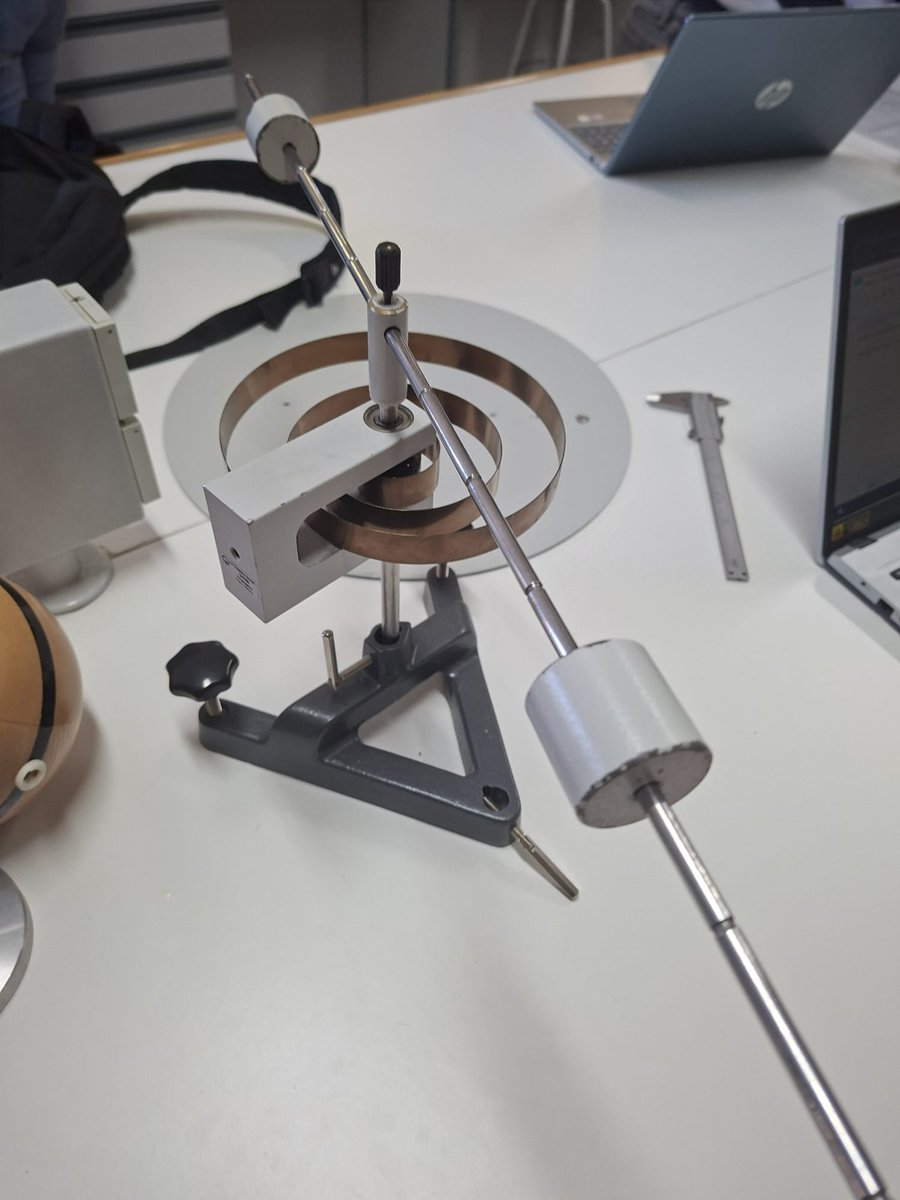
\includegraphics[width=\linewidth]{figuras/foto-varilla.jpg}\\[2pt]
  {\small\scshape (a)\; varilla}
\end{minipage}\hfill
\begin{minipage}[b]{0.235\textwidth}\centering
  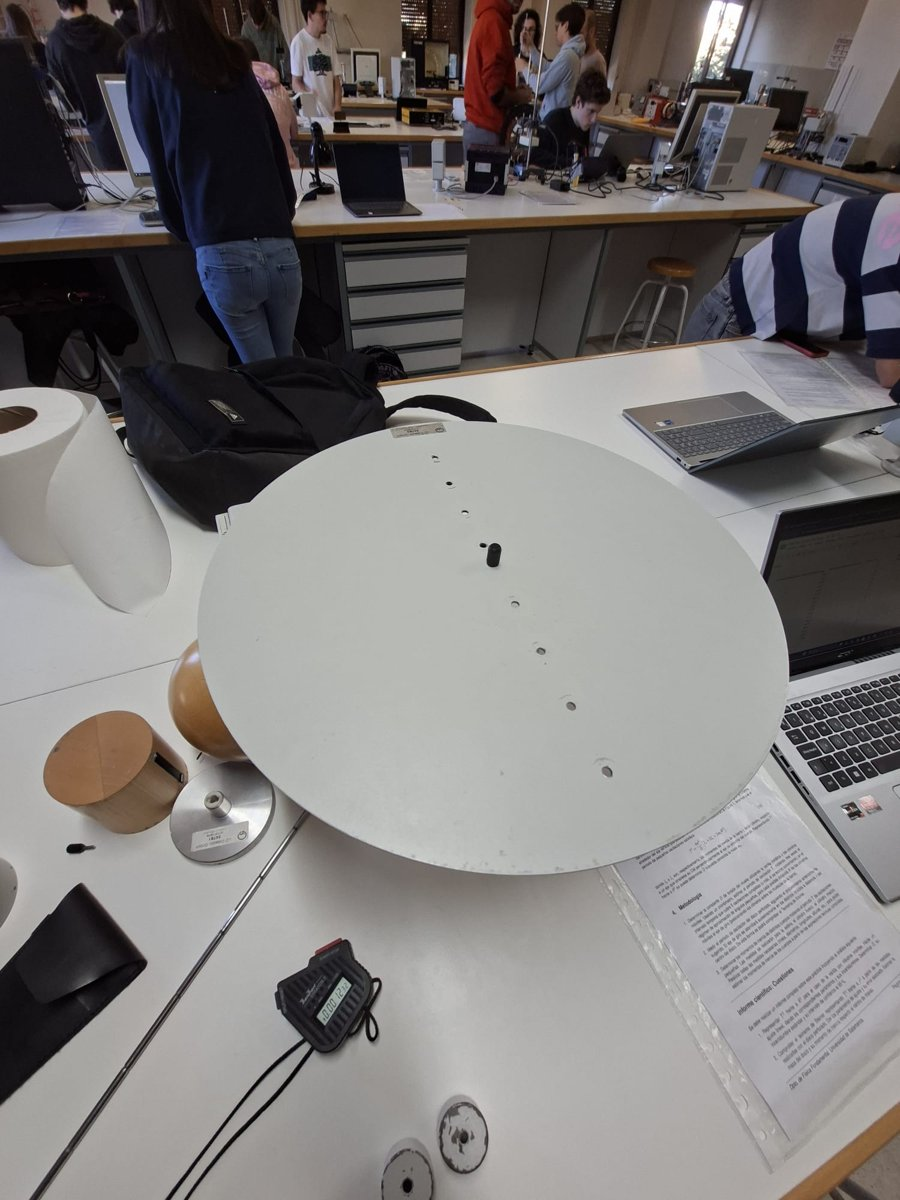
\includegraphics[width=\linewidth]{figuras/foto-disco.jpg}\\[2pt]
  {\small\scshape (b)\; disco}
\end{minipage}\hfill
\begin{minipage}[b]{0.235\textwidth}\centering
  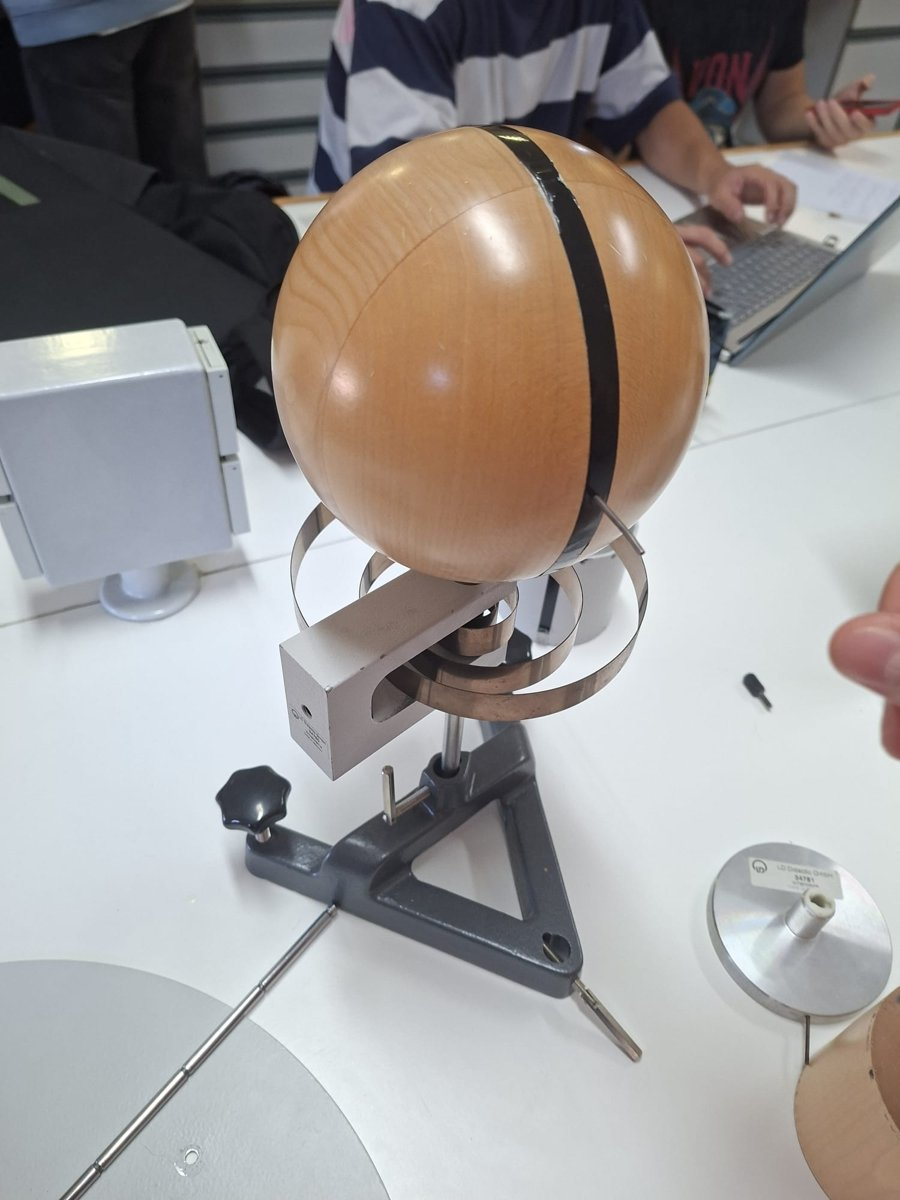
\includegraphics[width=\linewidth]{figuras/foto-esfera.jpg}\\[2pt]
  {\small\scshape (c)\; esfera}
\end{minipage}\hfill
\begin{minipage}[b]{0.235\textwidth}\centering
  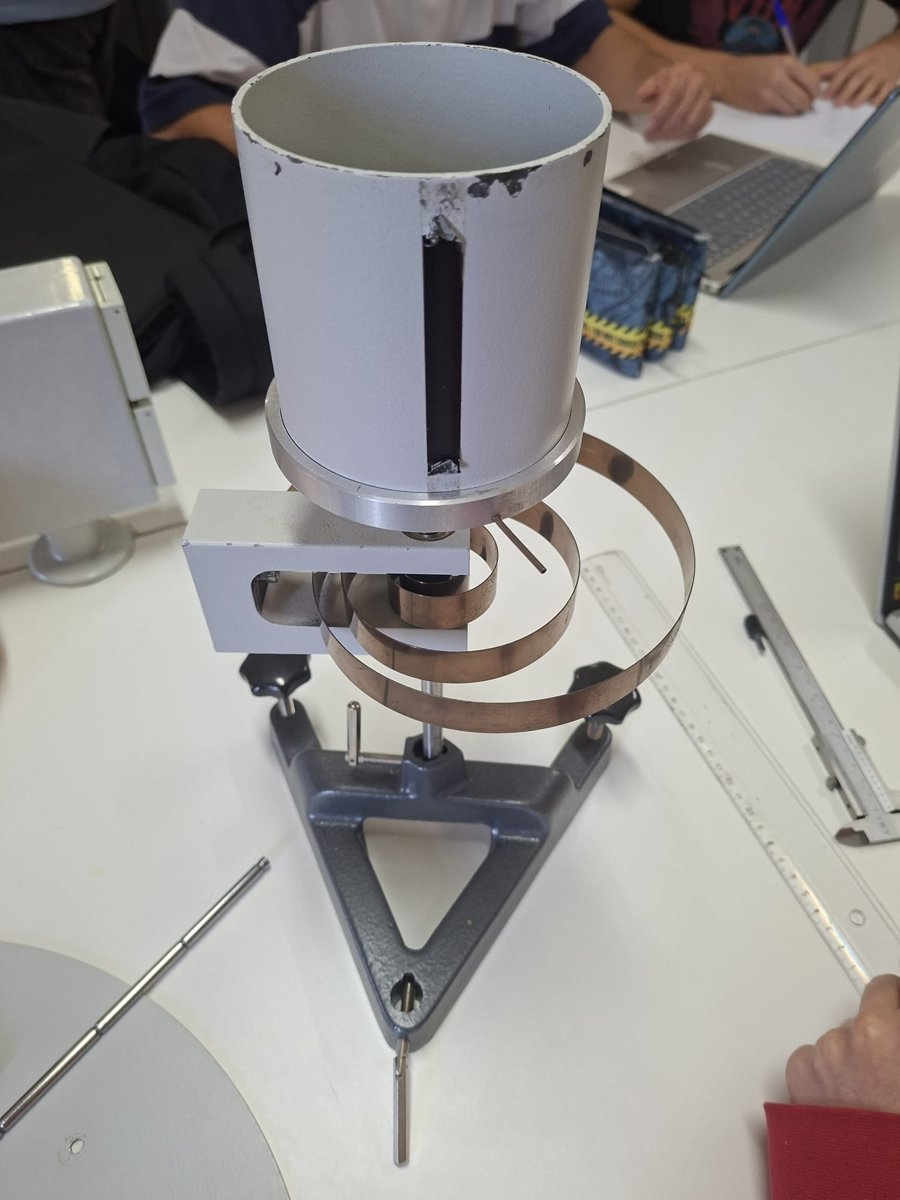
\includegraphics[width=\linewidth]{figuras/foto-cilindro-hueco.jpg}\\[2pt]
  {\small\scshape (d)\; cilindro hueco}
\end{minipage}
\caption{Configuraciones del péndulo de torsión en el laboratorio.
(a)~Varilla con los dos cilindros móviles, con la que calibramos el muelle.
(b)~Disco perforado, atornillado al eje por uno de sus orificios.
(c)~Esfera y (d)~cilindro hueco montados sobre el eje.}
\label{fig:fotos}
\end{figure}

\subsection{Montaje experimental}\label{sec:montaje}
El muelle espiral está sujeto por su extremo exterior a un soporte fijo
sobre un trípode, y por el interior a un eje vertical que puede girar
libremente; sobre el extremo superior del eje se atornillan los distintos
cuerpos (\cref{fig:montaje}). Al girar el eje un ángulo $\varphi$, el muelle
se enrolla o desenrolla y ejerce un momento recuperador que lo devuelve hacia
el equilibrio.

Con la varilla, los cilindros se colocan simétricamente sobre las muescas de
la barra, a una distancia $R$ del eje, de manera que el centro de masas del
conjunto sigue sobre el eje de giro. Con el disco, en cambio, el eje se
atornilla sucesivamente en orificios situados a distancias $r$ crecientes de
su centro: el disco gira entonces alrededor de un eje paralelo al que pasa
por su centro de masas, que es exactamente la situación que describe el
teorema de Steiner~\cite{GUION-P1}.

\begin{figure}[ht]
\centering
\begin{tikzpicture}[>=Stealth, x=0.62cm, y=0.62cm, font=\small]
  % ---------- (a) varilla con cilindros, en perspectiva ----------
  \begin{scope}
    \node[anchor=west, text=grispizarra] at (-7.4,6.2) {\small\scshape (a)\; varilla con cilindros};
    \def\phiM{24}\def\hM{2.5}\def\RM{4.6}\def\LM{6.9}
    \anillo[azulacero!70, line width=0.5pt, densely dotted]{\RM}{\hM}
    \draw[grispizarra!55, line width=0.6pt, dashed] (-\LM,\hM) -- (\LM,\hM);
    \draw[azulacero, line width=0.7pt, -{Stealth[length=4pt]}]
      plot[domain=2:\phiM-1.5, samples=30, variable=\t]
      ({6.2*cos(\t)},{\kp*6.2*sin(\t)+\hM});
    \node[azulprof] at ({6.85*cos(\phiM/2)},{\kp*6.85*sin(\phiM/2)+\hM+0.1}) {$\varphi$};
    \pendulotorsion{\phiM}{\hM}{\RM}{\LM}
    \draw[grispizarra, line width=0.45pt, |<->|]
      (0,\hM+1.3) -- ({-\RM*cos(\phiM)},{-\kp*\RM*sin(\phiM)+\hM+1.3})
      node[midway, above=1pt, text=azulprof, fill=white, inner sep=1.5pt] {$R$};
    \node[text=azulprof, anchor=west] at ({\RM*cos(\phiM)+0.5},{\kp*\RM*sin(\phiM)+\hM+0.85}) {$\mc$};
    \node[text=grispizarra, font=\itshape\footnotesize, anchor=west] at (4.7,-1.0) {muelle, $D$};
    \node[text=grispizarra, font=\itshape\footnotesize, anchor=east] at (-0.3,-2.2) {eje de giro};
  \end{scope}
  % ---------- (b) disco perforado, en planta ----------
  \begin{scope}[shift={(13.55,2.2)}]
    \node[anchor=west, text=grispizarra] at (-4.4,4.0) {\small\scshape (b)\; disco perforado (planta)};
    \draw[azulprof, fill=azulfondo, line width=0.7pt] (0,0) circle (3.5);
    % orificios a lo largo de un radio
    \foreach \x in {0.85,1.7,2.55}{\fill[white] (\x,0) circle (0.13); \draw[azulprof, line width=0.4pt] (\x,0) circle (0.13);}
    % centro de masas
    \draw[azulprof, line width=0.5pt, fill=white] (0,0) circle (0.2);
    \fill[azulprof] (0,0) circle (0.06);
    \node[azulprof, anchor=south east, inner sep=1pt] at (-0.12,0.15) {CM};
    % eje de giro en uno de los orificios
    \def\xA{1.7}
    \draw[acento, line width=0.8pt, fill=white] (\xA,0) circle (0.26);
    \draw[acento, line width=0.8pt] (\xA,0) ++(-0.18,-0.18) -- ++(0.36,0.36) ++(0,-0.36) -- ++(-0.36,0.36);
    \node[acento, anchor=north, inner sep=1pt, font=\footnotesize] at (\xA,-0.38) {eje};
    \draw[grispizarra, line width=0.45pt, |<->|] (0,-1.25) -- (\xA,-1.25)
      node[midway, below, text=azulprof] {$r$};
    \draw[grispizarra!50, line width=0.3pt, densely dotted] (\xA,-0.95) -- (\xA,-1.25);
    \draw[grispizarra!50, line width=0.3pt, densely dotted] (0,-0.25) -- (0,-1.25);
    % oscilación alrededor del eje
    \draw[azulacero, line width=0.7pt, {Stealth[length=4pt]}-{Stealth[length=4pt]}]
      ([shift={(\xA,0)}]45:0.8) arc[start angle=45, end angle=135, radius=0.8];
    \node[azulacero] at ([shift={(\xA,0)}]90:1.15) {$\varphi$};
    \node[text=grispizarra, font=\itshape\footnotesize] at (0,-2.55) {disco de masa $m$};
  \end{scope}
\end{tikzpicture}
\caption{Esquema del montaje. (a)~Péndulo de torsión con la varilla girada un
ángulo $\varphi$ respecto a su posición de equilibrio (discontinua); los dos
cilindros, de masa $\mc$, se sitúan simétricamente a una distancia $R$ del
eje. (b)~Disco perforado visto desde arriba: el eje de giro se atornilla en
un orificio a distancia $r$ del centro de masas, de modo que el disco oscila
alrededor de un eje paralelo al que pasa por su CM. Esquema sin escala.}
\label{fig:montaje}
\end{figure}

\ornamento

% =========================================================================
\newpage
\seccion{Fundamentos teóricos}{Del momento angular al periodo}\label{sec:fundamentos}
% =========================================================================
\subsection{Momento de inercia de un sólido rígido}\label{sec:momento}
Un sólido rígido es un sistema de partículas en el que la distancia entre
cualesquiera dos de ellas permanece constante~\cite{FI-DMG}. Si gira con
velocidad angular $\vect{\omega}$, cada partícula describe una circunferencia
alrededor del eje de giro, y su contribución a la inercia de la rotación
crece con el cuadrado de su distancia a ese eje.

\begin{definicion}[Momento de inercia respecto a un eje]\label{def:momento}
Sea $\rho_i$ la distancia de la partícula $i$, de masa $m_i$, al eje de giro.
El momento de inercia del sólido respecto a ese eje es
\begin{equation}\label{eq:momento}
  I=\sum_i m_i\,\rho_i^{2}
  \qquad\longrightarrow\qquad
  I=\int_{V}\rho_{\perp}^{2}\,\dif m=\int_{V}\rho_{\perp}^{2}\,\rho(\vect{r})\,\dif V,
\end{equation}
donde la segunda forma corresponde a una distribución continua de densidad
$\rho(\vect{r})$. Sus unidades en el SI son \si{\kilogram\meter\squared}.
\end{definicion}

En general, el momento angular y la velocidad angular no son paralelos: se
relacionan mediante una matriz simétrica, el tensor de inercia,
$\vect{J}=\mathsf{I}\,\vect{\omega}$, cuyos elementos diagonales son los
momentos de inercia respecto a los ejes coordenados y los no diagonales, los
productos de inercia~\cite{FI-FAB,FI-DMG}. Al ser simétrica, siempre existe
una base en la que es diagonal: la de los \emph{ejes principales de inercia}.

\begin{referencia}[Ejes principales de inercia]{FI-FAB}\label{ref:ejes}
Es fácil demostrar que cuando un sólido gira alrededor de un eje principal,
momento angular y velocidad angular son paralelos. [\dots] En sólidos
homogéneos y simétricos, los ejes principales coinciden con los ejes de
simetría del sólido.
\end{referencia}

En todas nuestras configuraciones el cuerpo gira alrededor de un eje de
simetría (la esfera, los cilindros, la varilla con los cilindros colocados
simétricamente) o de un eje paralelo a uno de simetría (el disco). En ese
caso el momento angular a lo largo del eje se reduce a
\begin{equation}\label{eq:J}
  J=I\,\omega=I\,\dot{\varphi},
\end{equation}
con $I$ un escalar: el momento de inercia respecto al eje de giro y
$\varphi$ el ángulo girado~\cite{GUION-P1}.

\subsection{El péndulo de torsión}\label{sec:torsion}
La variación del momento angular de un sólido está gobernada por el momento
resultante de las fuerzas exteriores, $\vect{M}=\dif\vect{J}/\dif t$. Para
un giro alrededor de un eje fijo y principal, su componente a lo largo del
eje, junto con la \cref{eq:J}, da la ecuación fundamental de la dinámica de
rotación~\cite{FI-FAB,GUION-P1}:
\begin{equation}\label{eq:dinamica}
  M=\ddt{J}=I\,\ddot{\varphi}.
\end{equation}
Es el análogo rotacional de $F=m\,a$: el momento de la fuerza ocupa el lugar
de la fuerza; la aceleración angular, el de la lineal, y el momento de
inercia, el de la masa.

Para ángulos pequeños, el muelle espiral responde como un resorte de torsión
lineal: ejerce un momento recuperador proporcional al ángulo girado, en una
ley de Hooke angular,
\begin{equation}\label{eq:hooke}
  M=-D\,\varphi,
\end{equation}
donde $D$ es la constante de torsión del muelle, en
\si{\newton\meter\per\radian}. Igualando las \cref{eq:dinamica,eq:hooke}
llegamos a la ecuación del movimiento,
\begin{equation}\label{eq:oscilador}
  \ddot{\varphi}+\frac{D}{I}\,\varphi=0,
\end{equation}
que es la de un oscilador armónico para la variable angular $\varphi$, con
solución general
\begin{equation}\label{eq:solucion}
  \varphi(t)=A\,\sin(\Omega t+\phi_0),
  \qquad
  \Omega^{2}\equiv\frac{D}{I},
\end{equation}
siendo $A$ la amplitud angular y $\phi_0$ la fase inicial, fijadas ambas por
las condiciones iniciales.

\begin{resultado}[Periodo de las oscilaciones de torsión]\label{res:periodo}
En la aproximación de pequeñas oscilaciones, un sólido de momento de inercia
$I$ respecto al eje de giro, acoplado a un muelle de constante de torsión
$D$, oscila con periodo
\begin{equation}\label{eq:periodo}
  T=\frac{2\pi}{\Omega}=2\pi\sqrt{\frac{I}{D}}
  \qquad\Longleftrightarrow\qquad
  I=\frac{D\,T^{2}}{4\pi^{2}},
\end{equation}
independiente de la amplitud.
\end{resultado}

Conocida $D$, medir el periodo equivale, por tanto, a medir el momento de
inercia. La relación es lineal entre $I$ y $T^{2}$, no entre $I$ y $T$; por
eso en todos los ajustes de este informe la variable dependiente será el
cuadrado del periodo.

\begin{observacion}[Límites del modelo]\label{obs:modelo}
La \cref{eq:periodo} descansa en tres aproximaciones que conviene tener
presentes al interpretar los datos. La primera es la linealidad del muelle,
que solo es razonable para amplitudes moderadas; por eso soltamos el sistema
desde ángulos pequeños. La segunda es despreciar el rozamiento en el eje y
con el aire: un amortiguamiento débil apenas modifica el periodo, pero sí
hace que la amplitud decaiga a lo largo de las oscilaciones que cronometramos.
La tercera es que $I$ debería incluir también la inercia de las piezas que
giran con el cuerpo (el propio eje, la tuerca y los soportes), $\Ie$, de
modo que en rigor $T^{2}=4\pi^{2}(I+\Ie)/D$. En las regresiones lineales esa
contribución constante queda absorbida en la ordenada en el origen y no
altera la pendiente; al medir sólidos aislados, en cambio, puede introducir
un pequeño sesgo sistemático que discutiremos con los datos.
\end{observacion}

\subsection{Teorema de Steiner}\label{sec:steiner}
Los momentos de inercia dependen del eje respecto al que se calculan. El
teorema de Steiner permite trasladarlos de un eje que pasa por el centro de
masas a cualquier otro paralelo a él~\cite{FI-FAB,FI-DMG}.

\begin{referencia}[Teorema de Steiner]{FI-FAB}\label{ref:steiner}
El momento de inercia $I_Z^{A}$ de un eje que pasa por un punto $A$ y que es
paralelo a un eje principal $Z$, de momento $I_Z^{\mathrm{CM}}$, es
$I_Z^{A}=I_Z^{\mathrm{CM}}+M D_Z^{2}$, siendo $D_Z$ la distancia entre
ambos ejes y $M$ la masa del sólido.
\end{referencia}

\begin{figure}[ht]
\centering
\begin{tikzpicture}[>=Stealth, scale=1.0, font=\small]
  % sólido arbitrario visto en la dirección de los ejes
  \draw[azulprof, line width=0.8pt, fill=azulfondo]
    plot[smooth cycle, tension=0.8] coordinates
    {(-2.6,0.2) (-1.9,1.6) (-0.2,2.1) (1.7,1.7) (2.9,0.6) (2.6,-1.0)
     (1.1,-1.8) (-0.9,-1.6) (-2.2,-1.1)};
  % ejes perpendiculares al papel
  \coordinate (CM) at (0.55,-0.35);
  \coordinate (A)  at (-1.55,-0.55);
  \coordinate (P)  at (0.95,1.45);
  \draw[azulprof, line width=0.6pt, fill=white] (CM) circle (0.17);
  \fill[azulprof] (CM) circle (0.05);
  \node[azulprof, anchor=north west] at ($(CM)+(0.05,-0.12)$) {CM};
  \draw[acento, line width=0.6pt, fill=white] (A) circle (0.17);
  \fill[acento] (A) circle (0.05);
  \node[acento, anchor=north] at ($(A)+(0,-0.2)$) {$A$};
  % elemento de masa
  \fill[azulacero] (P) circle (0.07);
  \node[azulacero, anchor=south west] at ($(P)+(0.03,0.03)$) {$\dif m$};
  % vectores (componentes perpendiculares a los ejes)
  \draw[->, line width=0.8pt, grispizarra] ($(A)!0.12!(CM)$) -- ($(A)!0.88!(CM)$)
    node[midway, below=1pt, text=black!80] {$\vect{d}$};
  \draw[->, line width=0.8pt, azulprof] ($(CM)!0.1!(P)$) -- ($(CM)!0.95!(P)$)
    node[midway, right=1pt, text=azulprof] {$\vect{s}_{\perp}$};
  \draw[->, line width=0.8pt, acento, densely dashed] ($(A)!0.07!(P)$) -- ($(A)!0.97!(P)$)
    node[pos=0.5, above left=0pt, text=acento] {$\vect{\rho}_{\perp}$};
  % leyenda
  \node[anchor=west, align=left, text=black!80] at (3.4,1.0)
    {$\vect{\rho}_{\perp}=\vect{d}+\vect{s}_{\perp}$};
  \node[anchor=west, align=left, text=black!80] at (3.4,0.2)
    {$\displaystyle\int\vect{s}_{\perp}\,\dif m=\vect{0}$};
  \node[anchor=west, align=left, text=black!80] at (3.4,-0.8)
    {$I_{A}=\Icm+M d^{2}$};
\end{tikzpicture}
\caption{Teorema de Steiner. Sección del sólido perpendicular a dos ejes
paralelos: uno pasa por el centro de masas (CM) y el otro por el punto $A$, a
distancia $d$. Un elemento de masa $\dif m$ dista $s_{\perp}$ del primero y
$\rho_{\perp}$ del segundo.}
\label{fig:steiner}
\end{figure}

\begin{teorema}[de Steiner o de los ejes paralelos]\label{teo:steiner}
Sea $\Icm$ el momento de inercia de un sólido de masa $M$ respecto a un eje
que pasa por su centro de masas, e $I_A$ el momento respecto a un eje paralelo
situado a distancia $d$. Entonces
\begin{equation}\label{eq:steiner}
  I_A=\Icm+M\,d^{2}.
\end{equation}
\end{teorema}

\begin{demostracion}
Tomemos ambos ejes perpendiculares al plano de la \cref{fig:steiner} y
llamemos $\vect{s}_{\perp}$ y $\vect{\rho}_{\perp}$ a las proyecciones, sobre
ese plano, de la posición de un elemento de masa $\dif m$ medida desde cada
eje; si $\vect{d}$ es el vector que va del eje $A$ al eje del CM,
$\vect{\rho}_{\perp}=\vect{d}+\vect{s}_{\perp}$. Llevándolo a la
\cref{eq:momento},
\begin{equation*}
  I_A=\int\rho_{\perp}^{2}\,\dif m
     =\int\bigl(d^{2}+2\,\vect{d}\cdot\vect{s}_{\perp}+s_{\perp}^{2}\bigr)\dif m
     =M d^{2}+2\,\vect{d}\cdot\!\int\vect{s}_{\perp}\,\dif m+\Icm .
\end{equation*}
La integral del término cruzado es nula por la propia definición de centro
de masas: medidas desde él, las posiciones de las masas se compensan. Queda
la \cref{eq:steiner}. \hfill$\square$
\end{demostracion}

El término $M d^{2}$ es el momento de inercia de una partícula de masa $M$
situada en el centro de masas: girar alrededor de un eje desplazado equivale
a girar alrededor del CM \emph{y}, además, a hacer orbitar toda la masa en
torno al nuevo eje~\cite{FI-FAB}. Como $M d^{2}\geq0$, el momento de
inercia es mínimo para el eje que pasa por el centro de masas, entre todos
los de una misma dirección.

Para el disco perforado, que oscila alrededor de un eje a distancia $r$ de su
centro de masas, las \cref{eq:periodo,eq:steiner} dan
\begin{equation}\label{eq:steinerT}
  T^{2}=\frac{4\pi^{2}}{D}\bigl(\Icm+m\,r^{2}\bigr)
       =\underbrace{\frac{4\pi^{2}\Icm}{D}}_{a}
       +\underbrace{\frac{4\pi^{2}m}{D}}_{b}\,r^{2}.
\end{equation}
El teorema de Steiner predice, por tanto, una dependencia \emph{lineal} de
$T^{2}$ con $r^{2}$. Si conocemos $D$, la pendiente y la ordenada de la recta
proporcionan la masa del disco y su momento de inercia respecto al CM:
\begin{equation}\label{eq:disco}
  m=\frac{D\,b}{4\pi^{2}},
  \qquad
  \Icm=\frac{D\,a}{4\pi^{2}}.
\end{equation}

\subsection{Calibración del muelle: varilla con cilindros móviles}\label{sec:calibracion}
Para conocer $D$ usamos el mismo razonamiento sobre un sistema cuyo momento
de inercia sabemos calcular: una varilla delgada de masa $\mb$ y longitud $L$
con dos cilindros iguales, de masa $\mc$, diámetro $d$ y altura $h$,
colocados simétricamente a una distancia $R$ del eje que pasa por el centro
de la varilla (\figpanel{fig:montaje}{a}). El centro de masas del conjunto
permanece sobre el eje y, aplicando el teorema de Steiner a cada cilindro,
\begin{equation}\label{eq:Ivarilla}
  I=\Ib+2\,\Ic+2\,\mc R^{2},
  \qquad
  \Ib=\frac{\mb L^{2}}{12},
  \qquad
  \Ic=\mc\left(\frac{d^{2}}{16}+\frac{h^{2}}{12}\right),
\end{equation}
donde $\Ib$ e $\Ic$ son los momentos de inercia de la varilla y de un
cilindro respecto a un eje que pasa por su CM perpendicularmente a su eje de
simetría~\cite{FI-FAB,GUION-P1}. El periodo cumple entonces
\begin{equation}\label{eq:varilla}
  T^{2}=\underbrace{\frac{4\pi^{2}}{D}\bigl(\Ib+2\Ic\bigr)}_{a'}
       +\underbrace{\frac{8\pi^{2}\mc}{D}}_{b'}\,R^{2},
\end{equation}
de nuevo lineal en el cuadrado de la distancia. Con la masa $\mc$ conocida,
la pendiente de la recta determina la constante de torsión,
\begin{equation}\label{eq:D}
  D=\frac{8\pi^{2}\mc}{b'},
\end{equation}
y la ordenada ofrece una comprobación independiente, pues debe ser
compatible con $4\pi^{2}(\Ib+2\Ic)/D$ calculada a partir de las dimensiones
de la varilla y de los cilindros.

\subsection{Momentos de inercia de sólidos sencillos}\label{sec:solidos}
Para los cuerpos homogéneos de geometría sencilla, la integral de la
\cref{eq:momento} puede resolverse de forma exacta. La \cref{tab:teoricos}
recoge las expresiones que necesitamos, todas respecto a ejes que pasan por
el centro de masas~\cite{ALONSO,FI-FAB,FI-DMG}.

\begin{table}[ht]
\centering
\caption{Momentos de inercia de sólidos homogéneos respecto a un eje que pasa
por su centro de masas. $M$ es la masa del sólido.}
\label{tab:teoricos}
\renewcommand{\arraystretch}{1.45}
\begin{tabular}{@{}l l l@{}}
\toprule
Sólido & Eje & Momento de inercia \\
\midrule
Esfera maciza de radio $R$            & cualquier diámetro                 & $\tfrac{2}{5}MR^{2}$ \\
Cilindro macizo (o disco) de radio $R$ & eje de simetría                   & $\tfrac{1}{2}MR^{2}$ \\
Cilindro hueco, radios $R_{1}<R_{2}$  & eje de simetría                    & $\tfrac{1}{2}M\bigl(R_{1}^{2}+R_{2}^{2}\bigr)$ \\
Cilindro hueco de pared delgada       & eje de simetría                    & $MR^{2}$ \\
Cilindro de radio $R$ y altura $h$    & perpendicular al eje de simetría   & $M\bigl(\tfrac{1}{4}R^{2}+\tfrac{1}{12}h^{2}\bigr)$ \\
Varilla delgada de longitud $L$       & perpendicular a la varilla         & $\tfrac{1}{12}ML^{2}$ \\
\bottomrule
\end{tabular}
\end{table}

Para cada uno de los tres sólidos dispondremos así de dos estimaciones del
momento de inercia: una \emph{dinámica}, a partir del periodo medido y de la
\cref{eq:periodo}, y otra \emph{geométrica}, a partir de su masa y sus
dimensiones con la \cref{tab:teoricos}. Compararlas mediante sus intervalos
de confianza al \SI{95}{\percent} es el último objetivo de la
práctica~\cite{GUION-P1}.

\ornamento

% =========================================================================
\newpage
\seccion{Procedimiento experimental}{Cómo medimos}\label{sec:procedimiento}
% =========================================================================
Seguimos la metodología del guion~\cite{GUION-P1}. En todos los casos
apartamos el sistema un ángulo pequeño de su posición de equilibrio, lo
soltamos sin impulso y, con el cronómetro, medimos tres veces el tiempo
$t_{n}$ que tarda en completar $n=\pend{5}$ oscilaciones. El periodo es
$T=t_{n}/n$.
\begin{enumerate}
  \item \emph{Calibración del muelle.} Con la varilla y los cilindros
        móviles colocados simétricamente sobre sus muescas, medimos el
        periodo para cada distancia $R$ disponible.
  \item \emph{Teorema de Steiner.} Atornillamos el eje sucesivamente en los
        orificios del disco perforado, a distancias $r$ de su centro, y
        medimos el periodo en cada uno.
  \item \emph{Sólidos.} Medimos el periodo de la esfera, el cilindro hueco y
        el cilindro macizo, y sus masas y dimensiones (diámetros, alturas y
        espesores) con el calibre y la regla.
\end{enumerate}
\pendiente{Describir aquí las particularidades de nuestra sesión: amplitud
aproximada de soltado, quién cronometró, criterio para iniciar y detener el
cronómetro, etc.}

\subsection{Tratamiento de incertidumbres}\label{sec:incertidumbres}
Seguimos la \emph{Guide to the expression of uncertainty in
measurement}~\cite{GUM}, tal como se recoge en las notas del
laboratorio~\cite{NUM-ARG}. Para una magnitud $y=f(x_1,\dots,x_N)$ con
entradas no correlacionadas, la incertidumbre típica se propaga como
\begin{equation}\label{eq:propagacion}
  u^{2}(y)=\sum_{k=1}^{N}\left(\frac{\partial f}{\partial x_k}\right)^{\!2}u^{2}(x_k),
\end{equation}
y la incertidumbre ampliada al \SI{95}{\percent} es $\ext{y}=\Tcoef\,u(y)$,
con $\Tcoef$ el factor de cobertura de Student para $\nu$ grados de
libertad~\cite{NUM-ARG}; el resultado se expresa como $y\pm\ext{y}$. Las
incertidumbres se dan con una sola cifra significativa, salvo cuando la
primera es un 1, en cuyo caso se conservan dos; el valor se redondea a la
misma posición decimal~\cite{ERR-MP}.

\begin{calculo}[Periodo de oscilación]\label{calc:T}
Para cada configuración, la media de las tres lecturas $t_{n,i}$ tiene una
incertidumbre de tipo~A, $u_A=s/\sqrt{3}$, con $s$ su desviación típica
muestral, a la que se suma en cuadratura la de tipo~B debida a la resolución
$\Delta$ del cronómetro, $u_B=\Delta/\sqrt{12}$~\cite{NUM-ARG,ERR-MP}.
Como $T=\mean{t}_{n}/n$ y la regresión se hace sobre $T^{2}$,
\begin{equation}\label{eq:uT}
  u(T)=\frac{u(\mean{t}_{n})}{n},
  \qquad
  u(T^{2})=2\,T\,u(T).
\end{equation}
Medir $n$ oscilaciones en lugar de una reduce la incertidumbre del periodo
en un factor $n$, porque los errores de arranque y parada del cronómetro
(dominados por el tiempo de reacción) se cometen una sola vez.
\end{calculo}

\begin{metodo}[Regresión lineal por mínimos cuadrados]\label{met:regresion}
Las \cref{eq:steinerT,eq:varilla} tienen la forma $y=a+b\,x$, con $y=T^{2}$
y $x=r^{2}$ o $x=R^{2}$. Para los $N$ pares $(x_i,y_i)$ ajustamos la recta
por mínimos cuadrados ordinarios, sin ponderar~\cite{NUM-ARG,HUGHES}. Con
$S_{xx}=\sum_i(x_i-\mean{x})^{2}$ y $S_{xy}=\sum_i(x_i-\mean{x})(y_i-\mean{y})$,
\begin{equation}\label{eq:regresion}
  b=\frac{S_{xy}}{S_{xx}},
  \qquad
  a=\mean{y}-b\,\mean{x},
  \qquad
  s^{2}=\frac{1}{N-2}\sum_{i=1}^{N}\bigl(y_i-a-b\,x_i\bigr)^{2},
\end{equation}
y las incertidumbres típicas de los parámetros son
\begin{equation}\label{eq:uregresion}
  u(b)=\frac{s}{\sqrt{S_{xx}}},
  \qquad
  u(a)=s\,\sqrt{\frac{1}{N}+\frac{\mean{x}^{2}}{S_{xx}}},
\end{equation}
con $\nu=N-2$ grados de libertad para construir los intervalos al
\SI{95}{\percent}. La calidad del ajuste la juzgamos con el coeficiente de
correlación lineal $r_{xy}$ y con la ausencia de tendencias en los
residuos.
\end{metodo}

\begin{calculo}[Constante de torsión]\label{calc:D}
Aplicando la \cref{eq:propagacion} a la \cref{eq:D},
\begin{equation}\label{eq:uD}
  \frac{u^{2}(D)}{D^{2}}=\frac{u^{2}(\mc)}{\mc^{2}}+\frac{u^{2}(b')}{b'^{2}}.
\end{equation}
Del mismo modo se propagan las incertidumbres de $m$ e $\Icm$ en la
\cref{eq:disco} y la de $I=DT^{2}/4\pi^{2}$ para cada sólido.
\end{calculo}

% =========================================================================
\newpage
\seccion{Análisis de datos y resultados}{Lo que dicen las medidas}\label{sec:analisis}
% =========================================================================
\pendiente{Sección pendiente de completar con los datos de la sesión.}

\subsection{Constante de torsión del muelle}\label{sec:resD}
Dimensiones y masas de la varilla y de los cilindros móviles:
$\mb=\pend{—}$, $L=\pend{—}$, $\mc=\pend{—}$, $d=\pend{—}$, $h=\pend{—}$.

\begin{table}[ht]
\centering
\caption{Tiempos de $n$ oscilaciones y periodos de la varilla con los
cilindros a distancia $R$ del eje.}
\label{tab:varilla}
\renewcommand{\arraystretch}{1.2}
\begin{tabular}{@{}c c c c c c@{}}
\toprule
$R$ (\si{\centi\meter}) & $t_{n,1}$ (\si{\second}) & $t_{n,2}$ (\si{\second}) &
$t_{n,3}$ (\si{\second}) & $T$ (\si{\second}) & $T^{2}$ (\si{\second\squared}) \\
\midrule
\pend{—} & \pend{—} & \pend{—} & \pend{—} & \pend{—} & \pend{—} \\
\pend{—} & \pend{—} & \pend{—} & \pend{—} & \pend{—} & \pend{—} \\
\pend{—} & \pend{—} & \pend{—} & \pend{—} & \pend{—} & \pend{—} \\
\bottomrule
\end{tabular}
\end{table}

\begin{figure}[ht]
\centering
\huecofigura{Gráfica de $T^{2}$ frente a $R^{2}$ con la recta de regresión
(\cref{eq:varilla}).}
\caption{Calibración del muelle: $T^{2}$ frente a $R^{2}$ para la varilla con
cilindros móviles.}
\label{fig:varilla}
\end{figure}

\begin{destacado}[Constante de torsión]
$D=\pend{—}\ \si{\newton\meter\per\radian}$ \quad (incertidumbre típica);
\quad intervalo al \SI{95}{\percent}: \pend{—}.
\end{destacado}

\subsection{Comprobación del teorema de Steiner}\label{sec:resSteiner}
La \cref{tab:disco} recoge los periodos del disco para cada posición del eje,
y la \cref{fig:disco}, la regresión de $T^{2}$ frente a $r^{2}$.
\begin{table}[ht]
\centering
\caption{Periodos del disco perforado con el eje a distancia $r$ de su
centro.}
\label{tab:disco}
\renewcommand{\arraystretch}{1.2}
\begin{tabular}{@{}c c c c c c@{}}
\toprule
$r$ (\si{\centi\meter}) & $t_{n,1}$ (\si{\second}) & $t_{n,2}$ (\si{\second}) &
$t_{n,3}$ (\si{\second}) & $T$ (\si{\second}) & $T^{2}$ (\si{\second\squared}) \\
\midrule
\pend{—} & \pend{—} & \pend{—} & \pend{—} & \pend{—} & \pend{—} \\
\pend{—} & \pend{—} & \pend{—} & \pend{—} & \pend{—} & \pend{—} \\
\pend{—} & \pend{—} & \pend{—} & \pend{—} & \pend{—} & \pend{—} \\
\bottomrule
\end{tabular}
\end{table}

\begin{figure}[ht]
\centering
\huecofigura{Gráfica de $T^{2}$ frente a $r^{2}$ con la recta de regresión
(\cref{eq:steinerT}).}
\caption{Teorema de Steiner: $T^{2}$ frente a $r^{2}$ para el disco
perforado.}
\label{fig:disco}
\end{figure}

\begin{destacado}[Disco perforado]
$m=\pend{—}$, \quad $\Icm=\pend{—}$.
\end{destacado}

\subsection{Momentos de inercia de los sólidos}\label{sec:resSolidos}
La \cref{tab:solidos} compara, para cada sólido, el momento de inercia
obtenido del periodo con el que predicen su masa y sus dimensiones.
\begin{table}[ht]
\centering
\caption{Momentos de inercia de los sólidos: valor dinámico, a partir del
periodo, y valor geométrico, a partir de la \cref{tab:teoricos}, con sus
intervalos al \SI{95}{\percent}.}
\label{tab:solidos}
\renewcommand{\arraystretch}{1.2}
\begin{tabular}{@{}l c c c@{}}
\toprule
Sólido & $T$ (\si{\second}) & $I_{\text{din}}$ (\si{\kilogram\meter\squared}) &
$I_{\text{geo}}$ (\si{\kilogram\meter\squared}) \\
\midrule
Esfera          & \pend{—} & \pend{—} & \pend{—} \\
Cilindro hueco  & \pend{—} & \pend{—} & \pend{—} \\
Cilindro macizo & \pend{—} & \pend{—} & \pend{—} \\
\bottomrule
\end{tabular}
\end{table}

% =========================================================================
\newpage
\seccion{Discusión y conclusiones}{Lo que aprendemos}\label{sec:discusion}
% =========================================================================
\pendiente{Sección pendiente: valor de $D$ y calidad de la calibración;
linealidad de $T^{2}$ frente a $r^{2}$ y compatibilidad de $m$ e $\Icm$ con
los valores esperados; comparación de los momentos de inercia dinámicos y
geométricos; fuentes de error (tiempo de reacción, amplitud, rozamiento,
inercia del eje).}

% =========================================================================
\newpage
%                              BIBLIOGRAFÍA
% =========================================================================
\printbibliography[title={Referencias}]

\end{document}
